\documentclass[11pt]{article}
\usepackage[preprint]{acl}
\usepackage{times}
\usepackage{latexsym}
\usepackage[T1]{fontenc}
\usepackage[utf8]{inputenc}
\usepackage{microtype}
% \usepackage{inconsolata} % available on Overleaf; not installed here
\usepackage{booktabs}
\usepackage{multirow}
\usepackage{xcolor}
\usepackage{amsmath}
\usepackage{graphicx}
\usepackage{xurl}

% Red box for the parts that still need the student's own results.
\newcommand{\todo}[1]{\par\noindent\fcolorbox{red}{red!6}{\parbox{\dimexpr\linewidth-2\fboxsep-2\fboxrule}{\small\raggedright\textcolor{red}{\textbf{TO COMPLETE:}} #1}}\par}
% Small boxed data snippet
\newcommand{\snip}[1]{\noindent\fbox{\parbox{\dimexpr\linewidth-2\fboxsep-2\fboxrule}{\footnotesize\raggedright\sloppy #1}}}

\title{Replicating and Extending Prefix-Tuning:\\ Table-to-Text Generation on E2E, ViGGO and a New Product-Description Dataset}

\author{Niharika Kunaminna \\
  Student ID 48930520 \\
  COMP8240 Applications of Data Science, Macquarie University \\
  \texttt{niharika.kunaminna@students.mq.edu.au}}

\begin{document}
\maketitle

\begin{abstract}
I replicate the table-to-text setting of prefix-tuning \citep{li-liang-2021-prefix}, which freezes a pretrained language model and trains only a short continuous prefix, and then test how far the method carries to new data. After five fixes to its 2021 environment, the authors' own code with GPT-2 medium reaches 67.4 BLEU on the E2E test set after one training epoch on a free Colab GPU (the paper uses five) and with the paper's general rather than its E2E-specific hyperparameters, 2.3 BLEU below the 69.7 reported. A lightweight reimplementation with GPT-2 small and Hugging Face \texttt{peft} on a laptop CPU reaches 57.1 BLEU and is used for the new-data experiments, so those results test this reimplementation rather than the authors' code. On ViGGO, an existing video-game dataset, a prefix warm-started from E2E beats one trained from scratch (38.3 vs.\ 32.7 BLEU, 91\% vs.\ 76\% slot coverage). On a new Flipkart product-description dataset that I built and annotated (131 pairs), the method largely fails (3.8 BLEU), and annotation shows why: most human descriptions contain facts that are not in the input. Two annotators agreed only slightly ($\kappa = 0.03$ over 100 pairs, no written guidelines). With written guidelines, agreement on 31 further pairs was substantial ($\kappa = 0.65$), but 30 and 29 of the 31 labels were \emph{no}, so this is not evidence that the guidelines work. An LLM-as-judge pass shows that word-overlap metrics and slot coverage miss many hallucinations.
\end{abstract}

\section{Description of the Paper and Justification}

\subsection{The paper}
Fine-tuning adapts a pretrained language model (LM) by updating all of its parameters, so a full copy of the model must be stored for each task. \citet{li-liang-2021-prefix} propose \emph{prefix-tuning}: the LM is frozen and a short sequence of continuous, task-specific vectors (the \emph{prefix}) is prepended to the activations at every transformer layer. Real tokens attend to the prefix as if it were a sequence of ``virtual tokens''. Only the prefix is trained, about 0.1\% of the parameters of the model. To stabilise training, the prefix is not optimised directly but produced by a small MLP from a smaller matrix; after training only the prefix is kept. The paper applies the method to table-to-text generation with GPT-2 \citep{radford-etal-2019-gpt2} and to summarisation with BART \citep{lewis-etal-2020-bart}.\footnote{Paper: \url{https://aclanthology.org/2021.acl-long.353/}; official code: \url{https://github.com/XiangLi1999/PrefixTuning}.}

\subsection{Evaluation framework and original results}
Table-to-text output is scored against human references with the official scripts of each benchmark: BLEU \citep{papineni-etal-2002-bleu}, NIST \citep{doddington-2002-nist}, METEOR \citep{banerjee-lavie-2005-meteor}, ROUGE-L \citep{lin-2004-rouge} and CIDEr \citep{vedantam-etal-2015-cider} for E2E, plus TER and learned metrics for WebNLG and DART; summarisation is scored with ROUGE-1/2/L. The paper compares prefix-tuning with full fine-tuning, fine-tuning only the top two layers, and adapter-tuning \citep{houlsby-etal-2019-adapters}.

With GPT-2 medium and 0.1\% of the parameters, prefix-tuning matched or beat fine-tuning on table-to-text: 69.7 vs.\ 68.2 BLEU on E2E, 46.4 vs.\ 46.2 on DART, and 55.1 vs.\ 46.5 BLEU on WebNLG overall, where the gain came mostly from categories unseen in training (45.6 vs.\ 27.7). On XSum it was slightly worse than fine-tuning (ROUGE-L 35.05 at 0.1\% and 36.05 at 2\% vs.\ 37.25). It also beat fine-tuning in low-data settings by 2.9 BLEU on average, and extrapolated better to unseen topics. Table~\ref{tab:e2e} lists the E2E numbers I compare against.

\subsection{Justification}
\paragraph{Venue.} ACL is the flagship venue of computational linguistics, ranked A* in the CORE conference rankings and the top Computational Linguistics venue in Google Scholar Metrics.\footnote{\url{https://portal.core.edu.au/conf-ranks/}; \url{https://scholar.google.com/citations?view_op=top_venues&vq=eng_computationallinguistics}.}
\paragraph{Impact.} The paper has over 8,000 citations on Google Scholar (checked 2 November 2026). It is one of the founding methods of parameter-efficient fine-tuning; later methods such as prompt tuning \citep{lester-etal-2021-power} and LoRA \citep{hu-etal-2022-lora} compare against it.
\paragraph{Reproducibility.} The authors released code, all four datasets are public with standard splits, and the method is reimplemented in the widely used Hugging Face \texttt{peft} library \citep{mangrulkar-etal-2022-peft}, which lowers the risk of the project.

\begin{figure*}[t]
\begin{minipage}[t]{0.49\textwidth}
\snip{\textbf{E2E (test)} \\
\texttt{name[The Vaults], eatType[restaurant], food[French], priceRange[moderate], area[riverside], familyFriendly[yes], near[Raja Indian Cuisine]}\\
\textit{Ref:} The Vaults is a reasonably priced, family friendly restaurant located near Raja Indian Cuisine by the river. \;(1 of 11 refs)\\
\textit{Ours:} The Vaults is a French restaurant near Raja Indian Cuisine. It is family friendly and has a moderate price range.}

\vspace{2pt}
\snip{\textbf{WebNLG (as included in the DART test set)} \\
\texttt{(Ab Klink | ALMA\_MATER | Erasmus University Rotterdam), (Ab Klink | PARTY | Christian Democratic Appeal), (Ab Klink | BIRTH\_PLACE | Netherlands)}\\
\textit{Ref:} Ab Klink was born in the Netherlands, belongs to the Christian Democratic Appeal party and graduated from Erasmus University in Rotterdam.}

\vspace{2pt}
\snip{\textbf{DART (test, from WikiTableQuestions)} \\
\texttt{(Hawaii Five-O | NOTES | Episode: The Flight of the Jewels), ([TABLECONTEXT] | [TITLE] | Jeff Daniels), ([TABLECONTEXT] | TITLE | Hawaii Five-O)}\\
\textit{Ref:} Jeff Daniels played in the Hawaii Five-O episode The Flight of the Jewels}

\end{minipage}\hfill
\begin{minipage}[t]{0.49\textwidth}
\snip{\textbf{ViGGO (test)} \\
\texttt{inform(name[The Witcher 3: Wild Hunt], developer[CD Projekt RED], esrb[M (for Mature)], rating[excellent], genres[action-adventure, role-playing])}\\
\textit{Ref:} The Witcher 3: Wild Hunt is CD Projekt RED's excellent action-adventure title. Rated M (for Mature), it has been universally praised for its role-playing elements. The game is available for PlayStation, Xbox, and PC.}

\vspace{2pt}
\snip{\textbf{Flipkart (new, train)} \\
\texttt{name[Nimya Solid Men's Polo Neck T-Shirt], category[Clothing], subcategory[Men's Clothing], priceRange[expensive], type[Polo Neck], ideal for[Men's], occasion[Casual], pattern[Solid]}\\
\textit{Ref:} Nimya Is In Lifestyle Fashion And Athletic Apparels. This Polo T-Shirt Is Made To Bring Out The Style In You. \;(annotated \textit{yes})}

\end{minipage}
\caption{Examples from the datasets: E2E (with my E2E model's output), WebNLG and DART triples from the paper, and the two datasets I added. XSum is not shown: each instance is a full BBC article (431 words on average) with a one-sentence summary. The ViGGO reference mentions platforms that are not in the MR.}
\label{fig:snippets}
\end{figure*}

\section{Datasets in the Original Paper}

\paragraph{E2E} \citep{novikova-etal-2017-e2e} is a crowdsourced restaurant-domain dataset of about 50K examples. Each input is a meaning representation (MR): a flat list of up to eight attribute--value pairs (\textit{name, eatType, food, priceRange, customer rating, area, familyFriendly, near}). Each MR has several human references; in the official split, 42,061 training pairs, 4,672 development pairs and 4,693 test pairs, where the test set has 630 distinct MRs (7.4 references each). Figure~\ref{fig:snippets} shows a test example.\footnote{\url{https://github.com/tuetschek/e2e-dataset}}

\paragraph{WebNLG} \citep{gardent-etal-2017-webnlg} has about 22K examples whose inputs are sets of RDF triples (\textit{subject | property | object}) taken from DBpedia, verbalised as one or more sentences. The test set is split into categories seen in training and five unseen categories, which is what allows the paper's extrapolation results.\footnote{\url{https://gitlab.com/shimorina/webnlg-dataset}}

\paragraph{DART} \citep{nan-etal-2021-dart} is an open-domain dataset of about 82K examples, also expressed as triples, built from Wikipedia tables (WikiSQL, WikiTableQuestions) together with converted E2E and WebNLG data.\footnote{\url{https://github.com/Yale-LILY/dart}}

\paragraph{XSum} \citep{narayan-etal-2018-dont} pairs about 225K BBC news articles (431 words on average) with one-sentence summaries (23.3 words), and is used for the BART summarisation experiments.\footnote{\url{https://github.com/EdinburghNLP/XSum}}



\section{Replication of the Original Work}

\paragraph{Scope.} I replicated the paper's E2E experiments only. E2E is the table-to-text benchmark the paper reports in most detail (all five metrics and the low-data experiments), and with roughly one training epoch per free Colab session, adding WebNLG, DART or the BART summarisation runs on XSum was not feasible. The replication has two parts: the authors' own code with GPT-2 medium (Section~\ref{sec:authors}), which tests whether the reported result can be reproduced, and a lightweight \texttt{peft} reimplementation with GPT-2 small (Section~\ref{sec:peft}), which runs on a laptop CPU and is the system used for the new-data experiments in Section~\ref{sec:newresults}.

\subsection{Running the authors' code}\label{sec:authors}
The specification asks for the original code on the original data. The official repository (branch \texttt{cleaned}) trains E2E prefixes with \texttt{gpt2/train\_e2e.py}, which builds a command for \texttt{run\_language\_modeling.py}, on top of a modified copy of \texttt{transformers} 3.2.0 bundled in the repository; \texttt{gen.py} and \texttt{run\_generation.py} then decode and call the official E2E scorer. I ran it on Google Colab with a T4 GPU (notebook \path{colab/original_code_run_with_outputs.ipynb}, with all cell outputs). Getting it to run took five fixes:
{\sloppy
\begin{enumerate}\setlength\itemsep{0pt}
\item Colab's Python 3.13 cannot build \texttt{tokenizers} 0.8.1rc2, which the bundled \texttt{transformers} requires. I created a Python 3.8.20 environment with \texttt{uv} and installed torch 1.13.1, the bundled library and \texttt{six}, which the library imports but does not declare.
\item \texttt{train\_e2e.py} launches training with \texttt{os.system("python \dots")}, which picked up Colab's own Python and current \texttt{transformers} (\texttt{ImportError: cannot import name 'cached\_path'}). I called the Python 3.8 interpreter directly.
\item Model cache, test data, output folder and scorer are hard-coded to the authors' servers (\texttt{/u/scr/xlisali/\dots}). I downloaded GPT-2 medium from Hugging Face and patched the paths.
\item \texttt{gen.py} infers its settings from the name of the model folder: a folder without \texttt{prefixtune} in its name crashes with \texttt{NameError: name 'tuning\_mode' is not defined}, and it always passes a prefix length of 20. I called \texttt{run\_generation.py} directly with the training settings.
\item \texttt{run\_generation.py} in turn reads the prefix format (\texttt{cat}, \texttt{peek}, \dots) from the folder name and otherwise stops with an \texttt{AssertionError}. I linked the model folder under a name containing \texttt{cat}.
\end{enumerate}
}
Training then ran with GPT-2 medium and the MLP reparameterisation (hidden size 512; 25,750,016 parameters during training). This run deviates from the paper's E2E configuration in two ways. It uses the paper's general table-to-text settings (its Section~5.3: learning rate $5\times10^{-5}$ with linear decay, batch size 5, prefix length 10) rather than the E2E-specific settings in its appendix Table~5 (learning rate $8\times10^{-5}$, batch size 10, prefix length 5), which I identified only after the run; and it trains for one epoch rather than five, because of Colab's session limits. Section~\ref{sec:howclose} treats both as untested causes of the remaining gap. A first 300-step test (1,500 examples, 3.6\% of an epoch) took about a minute; the full epoch over all 42,061 training pairs (8,413 steps) took 31 minutes on the T4, against about an hour for my much smaller CPU run, with the logged loss falling from 73.8 at step 500 to 28.8 at step 8,000 (the code logs a summed, not per-token, loss). After training only the prefix activations are needed: $10 \times 24 \times 2 \times 1024 = 491{,}520$ values, 0.14\% of GPT-2 medium.

\paragraph{Result.} Decoding the 630 test MRs with beam search (beam 5) and scoring with the same scorer as my \texttt{peft} runs gave \textbf{67.4 BLEU}, 7.24 NIST and 68.8 ROUGE-L (Table~\ref{tab:e2e}), 2.3 BLEU below the paper's 69.7, after one epoch where the paper's E2E run used five. Slot coverage was 98.3\%: the area appears in 97\% of outputs (544/558), food in 96\% and price in 95\%, against 23\%, 73\% and 62\% for my \texttt{peft} model. The authors' code therefore reproduces the paper closely, and the remaining gap is consistent with the shorter training and the different hyperparameters; Section~\ref{sec:howclose} shows that the scorer explains the NIST gap but not the BLEU gap.


\subsection{Reimplementation with \texttt{peft}}\label{sec:peft}
\paragraph{Environment.} All runs used a Windows laptop CPU (no GPU), Python 3.11 with torch 2.14.1, transformers 5.18.0, peft 0.21.2 and datasets 5.0.1. The university VM and Codespace planned in the proposal were not needed once the CPU run time was known (about one hour for the main E2E run). One practical issue: installing into the Microsoft Store Python failed with ``filename too long'', fixed by a virtual environment on a short path. Code and results are public.\footnote{\url{https://github.com/KunaminnaNiharika/prefix-tuning-replication}}

\paragraph{Setup.} \texttt{train\_prefix.py} wraps GPT-2 small (124M parameters) with \texttt{peft}'s \texttt{PrefixTuningConfig} and a 10-token prefix: 184,320 trainable of 124,624,128 parameters (0.148\%), close to the paper's 0.1\%. Each MR is linearised (\texttt{name : The Vaults | food : French | \dots ==>}) and the loss is computed on the reference tokens only. I trained on a random 4,000 of the 42,061 E2E training pairs for 2 epochs (batch 8, AdamW, learning rate $3\times10^{-2}$ with linear decay) and decoded greedily. A pilot on 1,000 pairs chose the learning rate: $10^{-2}$ gave 13.4 BLEU on 50 test MRs, $3\times10^{-2}$ gave 47.5. A larger run (8,000 pairs, 3 epochs) was stopped after 380 of 3,000 steps because it would have taken over two hours on the CPU.

\paragraph{Scoring.} I score all 630 distinct test MRs against all their references with my own scorer: NLTK BLEU, NIST and METEOR on lower-cased tokens, and \texttt{rouge\_score} ROUGE-L (best over references). CIDEr is not computed. A first evaluation on the first 200 test MRs gave 55.7 BLEU, but those MRs cover only 10 of the 18 restaurant names, so I re-scored the saved prefix on the full set. Re-running from the saved prefix reproduces the numbers exactly. I also report \emph{slot coverage}: the share of \textit{name, eatType, food, priceRange, area} and \textit{near} values that appear word for word in the output, computed the same way for the human references as a baseline.

\begin{table}[t]
\centering\small
\setlength{\tabcolsep}{2pt}
\begin{tabular}{@{}lrrrrr@{}}
\toprule
System & BLEU & NIST & MET & R-L & CIDEr \\
\midrule
\multicolumn{6}{@{}l}{\textit{Reported by \citet{li-liang-2021-prefix}}} \\
GPT-2 M, fine-tune & 68.2 & 8.62 & 46.2 & 71.0 & 2.47 \\
GPT-2 M, prefix 0.1\% & 69.7 & 8.81 & 46.1 & 71.4 & 2.49 \\
GPT-2 L, prefix & 70.3 & 8.85 & 46.2 & 71.7 & 2.47 \\
\midrule
\multicolumn{6}{@{}l}{\textit{This work (own scorer, see text)}} \\
GPT-2 M, orig.\ code, 1 ep. & 67.4 & 7.24 & 78.8$^\dagger$ & 68.8 & -- \\
GPT-2 S, \texttt{peft}, 0.15\% & 57.1 & 5.17 & 64.9$^\dagger$ & 59.4 & -- \\
\midrule
\multicolumn{6}{@{}l}{\textit{This work, official E2E scorer}} \\
GPT-2 S, \texttt{peft}, 0.15\% & 56.3 & 6.92 & 35.5 & 59.9 & 1.63 \\
\bottomrule
\end{tabular}
\caption{E2E test set (630 MRs). The first two rows of this work use my NLTK/\texttt{rouge\_score} scorer; the last row scores the same \texttt{peft} outputs with the official E2E scripts. The authors'-code outputs were not kept, so they could not be re-scored. $^\dagger$NLTK METEOR is not comparable with the official METEOR (it is higher here although every other metric is lower).}
\label{tab:e2e}
\end{table}

\begin{table}[t]
\centering\small
\setlength{\tabcolsep}{3pt}
\begin{tabular}{@{}lll@{}}
\toprule
Setting & Paper & This work \\
\midrule
Model & GPT-2 medium/large & GPT-2 small \\
Training pairs & 42,061 (all) & 4,000 (9.5\%) \\
Epochs / batch & 5 / 10 & 2 / 8 \\
Learning rate & $8\times10^{-5}$ & $3\times10^{-2}$ \\
Prefix length & 5 & 10 \\
MLP reparam. & yes & no (\texttt{peft} default) \\
Decoding & beam 5 & greedy \\
Scorer & official E2E & NLTK, rouge-score \\
Hardware & GPU & laptop CPU \\
\bottomrule
\end{tabular}
\caption{Differences between the paper's E2E setup (its appendix Table~5) and my \texttt{peft} run.}
\label{tab:settings}
\end{table}

\subsection{How close, and why not closer}
\label{sec:howclose}
With the authors' code the replication is close: 67.4 BLEU against 69.7, 7.24 NIST against 8.81, and 68.8 ROUGE-L against 71.4 (Table~\ref{tab:e2e}). Three differences remain: one training epoch instead of five, the general rather than the E2E-specific hyperparameters, and my scorer instead of the official E2E scripts \citep{dusek-etal-2020-e2e}. The authors'-code outputs were lost with the Colab session, so I measured the scorer difference on my own greedy \texttt{peft} outputs instead: the official script gives 56.3 BLEU and 6.92 NIST where my scorer gives 57.1 and 5.17 (ROUGE-L 59.9 vs.\ 59.4; \path{results/e2e_full/official_e2e_metrics.json}). Official NIST is 1.7 higher than mine, about the size of the NIST gap to the paper (7.24 vs.\ 8.81), so the NIST gap is most likely a scorer artefact. Official BLEU is 0.8 \emph{lower}, so the scorer does not explain the BLEU gap: if the same offset holds for the authors'-code output, it would score about 66.6 officially, two to three points below the paper. I attribute this gap to the shorter training and different hyperparameters, which I did not test. All results in this report are single runs with one random seed, so I cannot report run-to-run variance. I therefore interpret only the large differences (2.3 BLEU to the paper, 10.3 between the two systems, 5.6 from warm-starting on ViGGO) and treat differences below about one BLEU point as within noise.

My \texttt{peft} reimplementation is 12.6 BLEU, 3.6 NIST and 12.0 ROUGE-L below the paper. The method clearly works, since 0.15\% of the parameters turn a general LM into a fluent restaurant describer, but it is not a like-for-like replication. Table~\ref{tab:settings} lists the differences. Candidate causes, of which decoding (below) and the scorer were tested: (1) GPT-2 small has a third of the parameters of GPT-2 medium; (2) I used under a tenth of the training data for two of the paper's five epochs; (3) without the paper's MLP reparameterisation, training the prefix directly needed a learning rate more than two orders of magnitude higher, and the paper reports that direct optimisation is less stable and performs worse; (4) greedy decoding instead of beam search; (5) the scorer differs: tokenisation, NIST and METEOR implementations differ from the official E2E scripts \citep{dusek-etal-2020-e2e}, which is visible in METEOR being \emph{higher} than the paper's; on these outputs the official script gives 0.8 BLEU less but 1.7 NIST more than mine (above).

\begin{table}[t]
\centering\small
\begin{tabular}{@{}lrrr@{}}
\toprule
Slot & $n$ & Model & Human refs \\
\midrule
name, near & 630, 618 & 100\% & 100\% \\
eatType & 630 & 100\% & 98\% \\
food & 546 & 73\% & 88\% \\
priceRange & 480 & 62\% & 62\% \\
area & 558 & \textbf{23\%} & 78\% \\
\bottomrule
\end{tabular}
\caption{E2E slot coverage (value appears verbatim) on the 630 test MRs. With a looser check (``riverside'' or ``centre/center'' anywhere) area rises to 86\% for the references but stays at 23\% for the model.}
\label{tab:slots}
\end{table}

\paragraph{Decoding ablation.} To test one of these causes directly, I re-decoded the saved E2E prefix in a fresh Colab environment (T4 GPU, transformers 5.22.0, peft 0.21.2). Greedy decoding reproduced my laptop numbers exactly (57.1 BLEU), and beam search with 5 beams on the same prefix raised BLEU to 59.4 (+2.3), NIST to 6.06, ROUGE-L to 62.3 and slot coverage from 78.1\% to 83.2\%, with the area now mentioned in 45\% of outputs instead of 23\%. Decoding therefore explains about 2 of the 12.6 BLEU points; the remaining causes were not tested separately.

\paragraph{Error analysis.} Slot coverage (Table~\ref{tab:slots}) shows where the gap comes from: the model always copies the name, type and landmark but mentions the area in only 23\% of outputs, against 78\% for the human references, and often drops the food type. It also produces a fixed nonsense phrase, ``has a customer rating of no children'', in 21 of the 630 outputs (3.3\%), which merges \textit{familyFriendly[no]} with the rating template. Omissions make outputs shorter than the references, which both BLEU's brevity penalty and ROUGE-L's recall term penalise.

\section{Construction of New Data}

\subsection{Existing dataset: ViGGO}
ViGGO \citep{juraska-etal-2019-viggo} is a video-game dataset for conversational data-to-text generation: 6,900 MR--utterance pairs (5,103 / 714 / 1,083) over 14 game attributes, each MR wrapped in one of 9 dialogue acts (e.g.\ \textit{inform, request, verify\_attribute}). Its slot--value format is the same as E2E's, which makes it a clean test of transfer to a new domain; unlike E2E, about half of its utterances are questions. I downloaded it from the GEM release on Hugging Face (\texttt{GEM/viggo}; \citealp{gehrmann-etal-2021-gem}) with \texttt{get\_viggo.py}, linearised MRs as for E2E and dropped the dialogue-act wrapper except in one run. For CPU time I used 2,000 training pairs and the first 100 distinct test MRs.\footnote{\url{https://huggingface.co/datasets/GEM/viggo}}

\subsection{New dataset: Flipkart product descriptions}
\paragraph{Source.} The proposal planned a Kaggle e-commerce file, but its product-description field turned out to contain no text (\texttt{build\_dataset.py} is kept in the repository as a record). I therefore used a 1,000-product sample of the PromptCloud Flipkart product data, redistributed on Hugging Face\footnote{\url{https://huggingface.co/datasets/kenthua/flipkart-raw-demo}, from \url{https://www.kaggle.com/datasets/PromptCloudHQ/flipkart-products}} under CC BY-SA 4.0. Each product has a name, a category tree, a retail price in rupees, a free-text description and a list of specification key--value pairs.

\paragraph{Processing.} \texttt{build\_flipkart.py} turns each product into an E2E-style MR and a target sentence. The MR holds the name, brand, top two category levels, a price band (terciles: up to Rs.~799 \emph{cheap}, up to Rs.~1,500 \emph{moderate}, above that \emph{expensive}) and up to four specification slots, preferring the most frequent keys (\textit{type, ideal for, color, occasion, pattern}) so that slots are shared across products as in E2E. The target is the first two sentences of the description after removing the name line, price line, boilerplate and repeated lines. Table~\ref{tab:build} shows how 1,000 products became 131 pairs: most descriptions were pure sales text (``Buy \dots\ at Flipkart.com. Only genuine products'') or a dump of the specification table. The 131 pairs were split 105 / 13 / 13. Targets average 26.1 words and MRs 8.65 slots (E2E outputs average 22.9 tokens; \citealp{li-liang-2021-prefix}). Only 57.3\% of targets contain any MR value verbatim, which is the first sign that the data is weakly grounded. Figure~\ref{fig:snippets} shows an example.

\begin{table}[t]
\centering\small
\begin{tabular}{@{}lr@{}}
\toprule
Step & Products \\
\midrule
Raw sample & 1,000 \\
\quad description only sales boilerplate & $-596$ \\
\quad description is a spec dump & $-190$ \\
\quad cleaned description $>45$ words & $-22$ \\
\quad cleaned description $<8$ words & $-21$ \\
\quad duplicate target sentence & $-37$ \\
\quad no price & $-3$ \\
Usable pairs (train / dev / test 105 / 13 / 13) & 131 \\
After removing 9 pairs annotated \textit{no} & 122 \\
\bottomrule
\end{tabular}
\caption{Construction of the Flipkart dataset (\texttt{build\_log.json}).}
\label{tab:build}
\end{table}

\subsection{Human annotation and agreement}\label{sec:annotation}
Because Flipkart descriptions were written to sell, not to verbalise an MR, I annotated 100 randomly chosen pairs for whether the target is supported by its MR: \emph{yes} (no factual claim outside the MR), \emph{partial} (about the right product but adds facts, e.g.\ a colour or material not in the MR) or \emph{no} (nothing product-specific is supported), with a short note per row. The result was 25 yes, 66 partial and 9 no. The 9 \emph{no} pairs were removed (\texttt{filter\_by\_annotation.py}), leaving 98 / 12 / 12 pairs for the experiments. This filter relies on my labels alone; given the low agreement reported below, it is not a reliable filter, and 31 of the 131 pairs had not been annotated when the filter was applied (they were labelled later, see below). Of the 12 test pairs, 10 were in this annotation (9 \emph{partial}, 1 \emph{yes}) and 2 were not.

A second annotator labelled all 100 pairs independently in two batches of 50, with only the label names as instruction. Agreement was \emph{slight} \citep{landis-koch-1977} in both batches (Cohen's $\kappa = 0.03$ and $0.06$; \citealp{cohen-1960-kappa}) and over all 100 pairs ($\kappa = 0.03$, 30\% raw agreement; Table~\ref{tab:kappa}). The disagreement was not random, and its direction changed between batches: in the first, the second annotator labelled 13 of my 29 \emph{partial} pairs \emph{no} and 9 \emph{yes}; in the second, 22 of my 37 \emph{partial} pairs \emph{yes} and 8 \emph{no}. For example, ``\dots this black top will make you look elegant'' for an MR with no colour: I counted ``black'' as an unsupported fact, the second annotator judged the description as about the right product. With only the label names given, the boundary of \emph{partial} was undefined, so the annotation measured how differently two careful readers interpret an undefined label, not annotator carelessness.

\begin{table}[t]
\centering\small
\begin{tabular}{@{}lrrrr@{}}
\toprule
Pairs & $n$ & Raw agr. & $\kappa$ & 95\% CI \\
\midrule
First batch & 50 & 32\% & 0.03 & $-0.13$ to $0.19$ \\
Second batch & 50 & 28\% & 0.06 & $-0.07$ to $0.18$ \\
All & 100 & 30\% & 0.03 & $-0.07$ to $0.13$ \\
\midrule
With guidelines$^\ast$ & 31 & 97\% & 0.65 & $0.00$ to $1.00$ \\
\bottomrule
\end{tabular}
\caption{Agreement between the two annotators (yes / partial / no). First three rows: the first 100 Flipkart pairs, labelled with only the label names as instruction. $^\ast$Last row: the 31 remaining pairs, labelled with the written guidelines (\texttt{guideline\_round\_annotator1/2.csv}); 30 and 29 of the 31 labels were \emph{no}, see text. CI: bootstrap with 10{,}000 resamples of pairs (\texttt{agreement\_bootstrap.py}).}
\label{tab:kappa}
\end{table}

{\sloppy I then wrote one-page guidelines (Appendix~\ref{app:guidelines}; \path{docs/annotation_guidelines.md}), and both annotators used them to label the remaining 31 pairs, which had not been annotated before. Raw agreement rose to 97\% ($\kappa = 0.65$; Table~\ref{tab:kappa}), but this is not evidence that the guidelines work. The annotators labelled 30 and 29 of the 31 pairs \emph{no}, so $\kappa$ rests on one or two pairs and its 95\% interval spans 0.00 to 1.00. The two sheets' notes are closely similar in wording. Both annotators report that they labelled separately and by hand, so I treat the overlap as unexplained rather than as evidence of copying; I could not verify it further. The repository history for these two sheets begins with their upload on 7 November and does not show when or how they were filled in; each annotator keeps their original file. More importantly, the labels contradict the guidelines. Step~2 says that a description about the right product which adds an unsupported fact is \emph{partial}, and in at least 20 of the 31 pairs the annotators' own notes describe exactly that (for example, a diamond ring is supported but the number of diamonds and the carat weight are not), yet the pairs were labelled \emph{no}. Applied as written, most of these pairs would be \emph{partial}. The round therefore shows that the guidelines, as worded, did not fix the boundary between \emph{partial} and \emph{no}; a next version needs worked examples at that boundary and a short calibration round before labelling. My first-round labels were deliberately not revised. The 31-pair labels were not used to filter the data: these pairs stayed in the experiments (26 train, 3 dev, 2 test) even though 30 of my 31 labels for them are \emph{no}, which the filter would have removed, so the filtered data rests on the first 100 labels only.\par}


\section{Results on New Data}\label{sec:newresults}

\paragraph{System and evaluation.} All new-data experiments use the \texttt{peft} reimplementation (Section~\ref{sec:peft}), not the authors' code: the authors' code ran only in the patched Python 3.8 Colab environment, while the new-data runs, including the pilots and the warm start from the E2E prefix, were built on my \texttt{peft} script and run on the laptop CPU. This section therefore tests prefix-tuning as implemented in \texttt{peft}, which is 10.3 BLEU below the authors' code on E2E (57.1 vs.\ 67.4). The comparisons my conclusions rest on are within this one system (warm start vs.\ scratch, with and without the dialogue act, with and without the 3-gram constraint), so they do not depend on its absolute quality; the absolute ViGGO and Flipkart scores are probably lower than the authors' code would give. The evaluation also differs from the E2E replication: test sets are subsets (100 ViGGO MRs, 12 Flipkart MRs); each Flipkart MR has a single reference, whereas each E2E test MR has 7.4 on average, which lowers BLEU for the same output quality; and slot coverage is computed over different slots per dataset (Table~\ref{tab:new}). Decoding (greedy) and the scorer are the same as for the \texttt{peft} E2E run.

\begin{table}[t]
\centering\small
\setlength{\tabcolsep}{3pt}
\begin{tabular}{@{}llrrrrr@{}}
\toprule
Data & Prefix init. & BLEU & NIST & MET & R-L & Cov. \\
\midrule
E2E & scratch & 57.1 & 5.17 & 64.9 & 59.4 & 78.1 \\
\midrule
ViGGO & scratch & 32.7 & 3.79 & 48.4 & 44.9 & 76.2 \\
ViGGO & E2E & \textbf{38.3} & \textbf{4.54} & \textbf{53.5} & 47.4 & \textbf{91.2} \\
ViGGO & E2E + act & 37.0 & 4.42 & 53.3 & \textbf{49.2} & 82.3 \\
\midrule
Flipkart & scratch & 0.7$^\ast$ & 0.84 & 9.1 & 12.7 & 11.4 \\
Flipkart & E2E & 3.8 & 1.32 & 19.2 & 16.5 & 40.9 \\
Flipkart & E2E + NR3 & 4.1 & 1.46 & 19.6 & 16.6 & 40.9 \\
\bottomrule
\end{tabular}
\caption{Results with the same scorer as Table~\ref{tab:e2e}. ViGGO: 2,000 training pairs, 2 epochs, 100 test MRs; coverage over \textit{name, release\_year, developer}. Flipkart: 98 training pairs, 20 epochs, 12 test MRs. NR3: no repeated 3-gram within the generated text. $^\ast$Smoothed; unsmoothed BLEU is 0. Single runs.}
\label{tab:new}
\end{table}

\subsection{ViGGO}
\begin{figure}[t]
\centering
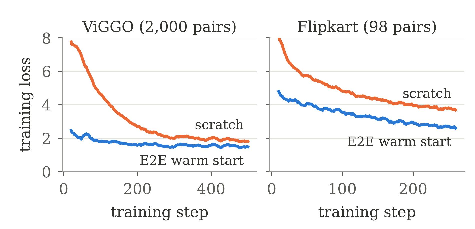
\includegraphics[width=\linewidth]{loss.pdf}
\caption{Training loss (moving average) for prefixes trained from scratch and warm-started from the E2E prefix.}
\label{fig:loss}
\end{figure}

ViGGO is harder than E2E for the same method (32.7 vs.\ 57.1 BLEU from scratch; Table~\ref{tab:new}), because many utterances are questions or opinions and references often add facts not in the MR (Figure~\ref{fig:snippets}). Starting from the E2E prefix instead of a random one starts training at a much lower loss (Figure~\ref{fig:loss}) and helps on every metric: +5.6 BLEU and +15 points of slot coverage, with release year covered in 97\% vs.\ 60\% and developer in 77\% vs.\ 40\%. The warm-started model also invents fewer ESRB ratings: among the 78 test MRs without an \textit{esrb} slot, 6 outputs mention a rating, against 21 for the cold start and 0 for the references. This is a small-scale echo of the paper's claim that prefixes transfer and extrapolate well. Giving the model the dialogue act raised the share of questions where the reference is a question (54\% to 67\%) and ROUGE-L, but lowered slot coverage (91\% to 82\%): the prefix trades content for form.

\subsection{Flipkart}
On Flipkart the method mostly fails: 3.8 BLEU with a warm start and essentially 0 from scratch. With only 98 training pairs the E2E warm start matters a great deal (coverage 41\% vs.\ 11\%), which is in line with the paper's low-data finding, but the outputs are poor. Four of the 12 cold-start outputs and 2 of the 12 warm-start outputs fall into repetition loops (``Brass, Brass, Brass, \dots''). I added a decoding constraint that forbids repeating any 3-gram \emph{within the generated text}; it removed all loops without hurting coverage. The built-in Hugging Face option (\texttt{no\_repeat\_ngram\_size}) could not be used because it also counts the prompt, which blocked copying the product name (name coverage 42\% to 0\%). With only 12 test MRs these scores are very noisy: differences of a few tenths of a BLEU point (3.8 vs.\ 4.1 with the 3-gram constraint) are within noise, and only the large gaps (coverage 41\% vs.\ 11\%, the loops) should be read as real. The main problem is the data, not the method: when two-thirds of the training targets add unsupported facts, the prefix learns to invent plausible product details, which the LLM judge confirms below.

\subsection{LLM-as-judge}
Word overlap cannot tell an omission from an invention, so I added an LLM judge as a second, faithfulness-oriented evaluation layer, with the slot coverage check as a cheap automatic proxy and human annotation as the reference point. The judge (Claude Opus 5.5, used through the Claude app on 2 November 2026) received each MR and output with a fixed rubric (Appendix~\ref{app:judge}) and returned: fluency (1--5), the number of MR values not expressed, whether any fact is invented or contradicted, whether the output repeats itself, and, for ViGGO, whether it fits the dialogue act. I sampled 40 E2E and 20 ViGGO outputs (random seed 1) and used all 12 Flipkart outputs of the warm-start run. All ratings are in \texttt{results/llm\_judge\_ratings.csv}.

\begin{table}[t]
\centering\small
\setlength{\tabcolsep}{3.5pt}
\begin{tabular}{@{}lrrrrr@{}}
\toprule
Data ($n$) & Fluency & Omit. & Halluc. & Repet. & Faithful \\
\midrule
E2E (40) & 4.55 & 1.62 & 12\% & 12\% & 8\% \\
ViGGO (20) & 3.90 & 1.05 & 40\% & 15\% & 25\% \\
Flipkart (12) & 2.58 & 2.08 & 58\% & 75\% & 0\% \\
\bottomrule
\end{tabular}
\caption{LLM-judge results. Omit.: mean MR values not expressed per output. Faithful: no omission and no hallucination. For Flipkart, omissions count only describable attributes (type, colour, material, pattern, occasion, brand).}
\label{tab:judge}
\end{table}

Table~\ref{tab:judge} ranks the three datasets in the same order as BLEU, but adds what the metrics hide. On E2E the outputs are fluent (4.55) but only 3 of 40 express every attribute: the judge counts all eight attributes, including \textit{customer rating} and \textit{familyFriendly}, which slot coverage ignores, so 75.5\% of all values are expressed against 81\% slot coverage on the same sample. Five E2E outputs hallucinate, e.g.\ an invented ``5 out of 5'' rating or ``low priced'' for \textit{customer rating[low]}. On ViGGO, slot coverage is 92\% on the sample, yet 8 of 20 outputs invent or contradict a fact (``developed by E 10+'', ``not available on PlayStation, Xbox or PC'' when the MR says it is), and the hallucinated outputs still have 88\% coverage: coverage simply cannot see added content. Some ViGGO inventions copy a habit of the references, which also mention platforms absent from the MR. Only 14 of 20 ViGGO outputs fit their dialogue act. On Flipkart no output is faithful; 7 of 12 invent details (a top described as ``casual jeans'', ``0.6 carat'' diamonds), which matches the human finding that most targets are only \emph{partially} supported.

The judge has clear limits, and I use it only as a diagnostic. It is a single model in a single pass, it has not been validated against human ratings of these outputs, and it was not blind to the aggregate metrics. It is also not independent of the project: the same assistant (Claude) ran the Colab replication and drafted this report, so it may share the report's expectations. For these reasons no conclusion in this report rests on the judge alone: the Flipkart conclusion rests on the human annotation (Section~\ref{sec:annotation}), and the ViGGO transfer result on BLEU and slot coverage (Table~\ref{tab:new}). The judge's role is to separate omission from hallucination and to name error types that slot coverage cannot see (invented ratings, platforms, diamond weights). Validating it would need human hallucination labels on the same outputs and a fresh session given only the rubric, MR and output.

\section{Ethical Considerations}

\paragraph{The original work.} Prefix-tuning lowers the storage and compute cost of adapting large models, which reduces energy use and makes adaptation accessible to groups without large hardware budgets; my whole project ran on a laptop CPU. The risks come from the frozen LM it relies on. GPT-2 was trained on web text and reproduces social biases \citep{sheng-etal-2019-woman}, and a frozen model keeps those biases because only the prefix is trained \citep{bender-etal-2021-parrots}. Data-to-text generation is used where readers trust the text to reflect a database, so hallucination \citep{ji-etal-2023-hallucination} is a harm in itself: my E2E and ViGGO outputs invent ratings and platforms. The paper evaluates with word-overlap metrics that are known to correlate weakly with human judgements \citep{novikova-etal-2017-need}, so reported gains need not mean more faithful text. Finally, its datasets were written by crowd workers, whose pay and conditions are not part of the paper.

\paragraph{Publishing on the new data.} The \emph{Australian Code for the Responsible Conduct of Research} \citep{nhmrc-2018-code} sets out principles that include honesty, rigour, transparency, fairness, respect, recognition and accountability, and responsibilities for data management, attribution and peer review. For this project they imply the following.
\textit{Attribution and licensing.} The Flipkart text was scraped from a commercial website and redistributed under CC BY-SA 4.0. Any release of my derived dataset must credit PromptCloud and the Hugging Face uploader and use the same ShareAlike licence, and the descriptions remain the sellers' and brands' text, not mine. The sellers wrote them to sell products, not expecting reuse as research data, and a licence on the redistributed copy does not settle whether the original collection respected Flipkart's terms of use, which I did not check and which would need checking before publication. A datasheet \citep{gebru-etal-2021-datasheets} should document the filtering, which removed 87\% of products and therefore biases the data towards categories with prose descriptions (clothing, jewellery).
\textit{Privacy.} The data holds product listings with brand names but no customer or personal data; this should be checked before release.
\textit{Human participants.} The second annotator is a human participant. A publication would need informed consent and, depending on the institution, ethics review under the National Statement on Ethical Conduct in Human Research \citep{nhmrc-2023-national}, even for this low-risk task.
\textit{Honest reporting.} Rigour and honesty mean reporting the low agreement and the failed Flipkart results rather than tuning until they look good, and not re-labelling pairs after seeing the disagreement.
\textit{Downstream harm.} A model trained on this data invents product facts such as diamond weights. Deployed in a shop, it could produce misleading product claims, so the data is suitable for studying unfaithfulness, not for training a production system.
\textit{AI use.} The unit allows AI use; the LLM judge and AI writing assistance are disclosed in this report, and I remain responsible for every claim and reference.

\section{Conclusions and Reflections}
The replication largely succeeded, within clear limits. Once five environment problems were fixed, the authors' own code trained a GPT-2 medium prefix in 31 minutes on a free Colab GPU and reached 67.4 BLEU on E2E after one epoch, against 69.7 in the paper after five. My lightweight \texttt{peft} reimplementation on GPT-2 small and a laptop CPU reached 57.1 BLEU; the gap to the authors' code has identifiable causes (model size, training budget, no MLP reparameterisation, greedy decoding) and is concentrated in dropped attributes, above all the area (23\% vs.\ 97\% coverage). Its limits are that only E2E was replicated, the authors'-code run used one epoch and the general hyperparameters, its outputs were not kept, and every result is a single run. Most of the effort of replicating a five-year-old codebase went into its environment and into settings hidden in folder names, not into the method.

The method generalises well to a structurally similar new domain: on ViGGO, in my \texttt{peft} reimplementation, an E2E-trained prefix transfers and beats a fresh one on every metric. It does not generalise to my product data, but the reason is the data. Annotation and the LLM judge both show that the targets are written to sell, not to describe the MR.

Three reflections. First, dataset construction mattered more than any model choice. A better design would pair each product with a description written or edited to match its MR, as E2E's crowd workers did, even at a much smaller size. Second, annotation was harder than expected: an undefined \emph{partial} label gave $\kappa = 0.03$ over 100 pairs, and guidelines should be written and piloted before annotation, not after, as I did. Third, faithfulness needs its own evaluation. BLEU, ROUGE and even slot coverage reward copying and miss invention, while an LLM judge exposed hallucinations that no automatic metric I computed could see.

\section*{Acknowledgements and Use of AI}
{\sloppy I thank the second annotator, who labelled all 131 Flipkart pairs: the first 100 in two batches of 50 with only the label names, and the remaining 31 with the written guidelines. I chose the paper and the project design, ran all \texttt{peft} experiments, built the Flipkart data and annotated all 131 pairs (100 with only the label names, 31 with the guidelines), and checked the numbers and the text. Generative AI (Claude, Anthropic) was used as permitted for this assessment: at my request it wrote the code for the \texttt{peft} experiments and data handling (\texttt{train\_prefix.py}, \texttt{build\_flipkart.py}, \texttt{filter\_by\_annotation.py} and the evaluation and agreement scripts), ran the Colab replication of the authors' code in my browser session (Section~3.1), produced the LLM-judge ratings (Section~5.3), wrote \texttt{score\_authors\_output.py} and the Colab notebook, and drafted the text of this report from my results. I have read every cited work.\par}

\bibliography{references}

\appendix

\section{LLM-Judge Rubric}
\label{app:judge}
\small
The judge was not run through an API with a stored prompt: Claude (Opus 5.5) rated the 72 outputs interactively in a chat session on 2 November 2026, given the MR, the output and the rubric below, which is therefore the complete instruction. No sampling settings apply, and there is no separate prompt file or screenshot; the ratings and a note for each are in \path{results/llm_judge_ratings.csv}.
For each item the judge saw the MR and the generated text and answered: (1) \textbf{Fluency} 1--5: 5 natural and grammatical; 3 understandable but awkward or repetitive; 1 broken or looping. (2) \textbf{Omitted values}: how many MR values the text does not express (E2E/ViGGO: every slot; Flipkart: type, colour, material, pattern, occasion, brand). (3) \textbf{Hallucination} yes/no: the text states a fact that is absent from or contradicts the MR (opinion words such as ``stylish'' do not count). (4) \textbf{Repetition} yes/no: a phrase or fact is repeated. (5) \textbf{ViGGO only, act fit} yes/no: questions for \textit{request, verify\_attribute, suggest, confirm}; an opinion for \textit{give\_opinion}; a statement for \textit{inform}. A short justification was recorded for every judgement that was not perfect.

\section{Annotation Guidelines (written after the first round; used for the 31-pair round)}
\label{app:guidelines}
Read the MR and the description. Step 1: if the description does not mention the product (its type, name or brand), label \textbf{no}. Step 2: if it states any concrete fact absent from the MR (colour, material, number, size, feature, origin), label \textbf{partial}. Step 3: otherwise label \textbf{yes}; opinion words alone do not make a description partial. Give a short reason in the notes, and label without seeing the other annotator's labels. Examples from the labelled pairs: ``\dots this black top will make you look elegant'' with no colour in the MR is \emph{partial}; ``The countdown is on! Time to select gifts \dots'' is \emph{no}.

\section{Reproducing the Results}
\label{app:repro}
The authors'-code run, with its training log, timings and scores, is in \path{colab/original_code_run_with_outputs.ipynb} (Colab, T4 GPU); \path{colab/original_code_attempt.ipynb} is the same code without outputs. The main \texttt{peft} commands are below; the README lists the commands for every other run (ViGGO, Flipkart, the beam-search ablation, the official-scorer check \texttt{official\_e2e\_scores.py}, \texttt{score\_authors\_output.py}), and each run's exact arguments are stored in \path{results/<run>/results.json}.
{\scriptsize
\begin{verbatim}
pip install -r requirements.txt
git clone https://github.com/tuetschek/e2e-dataset \
  data/e2e
python src/train_prefix.py \
  --train_csv data/e2e/trainset.csv \
  --test_csv data/e2e/testset_w_refs.csv \
  --n_train 4000 --epochs 2 --lr 0.03 \
  --prefix_len 10 --n_eval 200 \
  --out_dir results/e2e_short
python src/train_prefix.py \
  --train_csv data/e2e/trainset.csv \
  --test_csv data/e2e/testset_w_refs.csv \
  --init_adapter results/e2e_short/adapter \
  --epochs 0 --n_train 8 --n_eval 630 \
  --out_dir results/e2e_full
python src/agreement_bootstrap.py \
  data/newdata/annotation_sheet.csv \
  data/newdata/rater2_batch1.csv \
  data/newdata/rater2_batch2.csv
\end{verbatim}
}
\end{document}
